\documentclass[11pt,a4paper]{article}

\usepackage[margin=1in]{geometry}
\usepackage[T1]{fontenc}
\usepackage[utf8]{inputenc}
\usepackage{lmodern}
\usepackage{microtype}
\usepackage{hyperref}
\usepackage{amsmath}
\usepackage{enumitem}
\usepackage{booktabs}
\usepackage{array}
\usepackage{graphicx}
\usepackage{float}
\usepackage{xcolor}
\usepackage{tabularx}

\graphicspath{{../assets/}{assets/}{figures/}}

\title{CRISP-DM Report: Predicting Pull Request Merge Outcomes from GH Archive Events}
\author{%
    Nikita Zagainov\\
    \href{mailto:n.zagainov@innopolis.university}{n.zagainov@innopolis.university}\\
    Data Scientist, ML Engineer
    \and
    Dmitry Tetkin\\
    \href{mailto:d.tetkin@innopolis.university}{d.tetkin@innopolis.university}\\
    Business Unit, Project Manager, Business Analyst
}
\date{May 2026}

\setlist[itemize]{noitemsep, topsep=2pt}
\setlist[enumerate]{noitemsep, topsep=2pt}

\begin{document}
\maketitle

\section*{Group Roles and Work Distribution}

\begin{table}[H]
    \centering
    \small
    \caption{Group roles, responsibilities, and contribution summary.}
    \begin{tabularx}{\textwidth}{p{0.20\textwidth}p{0.22\textwidth}XX}
        \toprule
        Group member & Assigned role(s) & Main responsibilities & Contribution summary \\
        \midrule
        Nikita Zagainov
        & Data Scientist (0.5); ML Engineer (0.5)
        & Data extraction, feature construction, model implementation, tuning, evaluation, and technical reporting.
        & Built the PR-level analytical dataset, implemented the modeling pipeline, compared models, generated evaluation artifacts, and documented technical results. \\
        Dmitry Tetkin
        & Business Unit (0.33); Project Manager (0.34); Business Analyst (0.33)
        & Business framing, project coordination, stakeholder interpretation, recommendations, presentation planning, and video delivery.
        & Defined the business motivation, coordinated deliverable structure, interpreted results from a practical triage perspective, and prepared non-technical communication materials. \\
        \bottomrule
    \end{tabularx}
\end{table}

\section{Business Understanding (CRISP-DM Phase 1)}

\subsection{Determine Business Objectives (1.1)}

\subsubsection*{Background}

Open-source software development on GitHub depends heavily on pull requests (PRs) as the main mechanism for proposing, reviewing, and integrating code changes. Maintainers often need to prioritize review attention, while contributors benefit from understanding which early signals are associated with successful integration. Public GitHub event data captures observable workflow signals such as PR opening, PR closure, repository activity, actor activity, comments, pushes, and other event types. It does not capture private repository activity, full maintainer discussions, continuous integration results, or subjective review reasoning. Therefore, the project focuses on observable public signals rather than attempting to fully reproduce human maintainer decisions.

The project studies \textbf{pull request merge outcome prediction}. The analytical objective is to estimate whether a PR will eventually be merged using information available at the moment of PR publication and repository or actor activity observed before the opening day.

\subsubsection*{Business Objectives}

\begin{itemize}
    \item Identify early PR-level, repository-level, and contributor-level signals associated with merge outcomes.
    \item Build a reproducible model that ranks newly opened PRs by merge likelihood or non-merge risk.
    \item Provide an interpretable analytical basis for maintainer triage and contributor guidance.
\end{itemize}

\subsubsection*{Business Success Criteria}

\begin{itemize}
    \item The model should improve over a trivial majority-class baseline.
    \item The model should provide useful ranking quality for high-confidence merge or non-merge prioritization.
    \item The feature set should avoid post-publication leakage and remain explainable to non-technical stakeholders.
    \item The final conclusions should clearly separate predictive association from causal explanation.
\end{itemize}

\subsection{Assess Situation (1.2)}

\subsubsection*{Inventory of Resources}

\paragraph{People.}
\begin{itemize}
    \item Data Scientist / ML Engineer: data extraction, feature construction, modeling, evaluation, and report preparation.
    \item Business Unit / Project Manager / Business Analyst: business framing, stakeholder interpretation, and presentation/video delivery.
\end{itemize}

\paragraph{Data.}
The project uses a local sample of GH Archive hourly event records from July 2015. The raw data consists of compressed JSON-lines archives of public GitHub events. These records were converted into a flat analytical event table for efficient inspection and modeling. The converted event table contains 9,269,533 public GitHub events.

\paragraph{Tools.}
Python, Polars, pyarrow, scikit-learn, a notebook environment, and matplotlib were used. Polars was used for event processing and feature construction, while scikit-learn was used for model fitting and evaluation.

\subsubsection*{Requirements, Assumptions, and Constraints}

\paragraph{Requirements.}
\begin{itemize}
    \item Use only public event data available from GH Archive.
    \item Construct a reproducible PR-level modeling table.
    \item Avoid target leakage from PR closure or future activity.
    \item Report results using classification and ranking metrics rather than accuracy alone.
\end{itemize}

\paragraph{Assumptions.}
\begin{itemize}
    \item Public GitHub events are sufficiently informative to capture part of the PR merge process.
    \item A closed PR with \texttt{pull\_request.merged=true} represents successful integration.
    \item Historical repository and actor activity observed before the PR opening day can be used as context available at publication time.
\end{itemize}

\paragraph{Constraints.}
\begin{itemize}
    \item The data window is limited, so repository and actor histories are left-censored at the beginning of the sample.
    \item Only PRs whose opening and closing events are both observed in the downloaded window can receive a clean supervised label.
    \item GH Archive stores event payloads with event-specific JSON schemas, so not all potentially useful GitHub fields are uniformly available.
    \item The analysis is offline and cannot validate real maintainer decisions through live A/B testing.
\end{itemize}

\subsubsection*{Risks and Contingencies}

\begin{itemize}
    \item \textbf{Target leakage risk.} Closure-time fields may accidentally enter the feature matrix. Mitigation: exclude closure timestamps, raw merge labels, time-to-close diagnostics, and closure event identifiers from model features.
    \item \textbf{Sample bias risk.} Requiring both opening and closing events favors PRs that complete inside the observation window. Mitigation: interpret the task as short-window observable-lifecycle PR modeling and document this limitation.
    \item \textbf{Class imbalance risk.} Most observed PRs are merged. Mitigation: compare against a majority baseline and use PR-AUC, ROC-AUC, precision@k, and risk-ranking metrics.
    \item \textbf{Historical truncation risk.} Early-window PRs have incomplete prior history. Mitigation: use conservative previous-day history features and state this as a limitation.
\end{itemize}

\subsubsection*{Terminology}

\begin{table}[H]
\centering
\caption{Project terminology.}
\begin{tabularx}{\textwidth}{lX}
\toprule
Term & Meaning \\
\midrule
GH Archive & Public archive of GitHub event stream records. \\
Pull request & GitHub object proposing code changes to a repository. \\
Merged PR & Closed PR whose payload reports \texttt{pull\_request.merged=true}. \\
Non-merged PR & Closed PR whose payload reports \texttt{pull\_request.merged=false}. \\
Risk score & \(1 - P(\text{merged})\), used to rank PRs by non-merge risk. \\
Actor history & Aggregated previous public activity of the PR opener. \\
Repository history & Aggregated previous public activity of the target repository. \\
\bottomrule
\end{tabularx}
\end{table}

\subsubsection*{Costs and Benefits}

The main project cost is analyst and engineering time required to acquire event archives, convert nested event records into analytical tables, construct a PR-level supervised dataset, and evaluate models. No paid data sources or commercial software were required. The potential benefit is an interpretable prioritization signal for maintainers: instead of treating all newly opened PRs equally, a dashboard or report could highlight PRs with unusually high non-merge risk for earlier inspection. In the course setting, the benefit is analytical rather than directly financial.

\subsection{Determine Data Mining Goals (1.3)}

\subsubsection*{Data Mining Goals}

\begin{itemize}
    \item Convert public GitHub event streams into a PR-level supervised learning dataset.
    \item Predict whether a PR will be merged as a binary classification task.
    \item Compare simple and non-linear models under the same train/test design.
    \item Identify which pre-opening signals contribute most to merge-outcome ranking.
\end{itemize}

\subsubsection*{Data Mining Success Criteria}

\begin{itemize}
    \item Improve ROC-AUC and PR-AUC over the majority-class baseline.
    \item Improve top-k ranking quality over the baseline merge rate.
    \item Identify high-risk non-merged PRs with precision meaningfully above the base non-merge rate.
    \item Keep all features compliant with information available at PR publication time.
\end{itemize}

\subsection{Produce Project Plan (1.4)}

\subsubsection*{Project Plan}

\begin{table}[H]
\centering
\small
\caption{Project stages, activities, and outputs.}
\begin{tabularx}{\textwidth}{lXXl}
\toprule
Stage & Key activities & Outputs & Est. time \\
\midrule
Data Understanding & Convert raw events, inspect event types and PR payloads & Event and PR summaries & 5 days \\
Data Preparation & Extract PR lifecycles, construct target, build safe features & PR-level dataset & 10 days \\
Modeling & Train baseline and stronger classifiers & Candidate models & 7 days \\
Evaluation & Compare metrics, inspect ranking quality and limitations & Final conclusions & 5 days \\
Deployment & Organize report, code, and recommended use scenario & Course deliverable & 3 days \\
\bottomrule
\end{tabularx}
\end{table}

\subsubsection*{Initial Assessment of Tools and Techniques}

Polars was selected for event processing because the raw archive contains millions of JSON-line records and requires efficient columnar aggregation. Scikit-learn was selected for modeling because the task is tabular binary classification and the course objective emphasizes interpretable baselines and reproducible evaluation. Logistic regression was selected as a linear baseline, while random forest and histogram-based gradient boosting were selected as stronger non-linear alternatives.

\clearpage
\section{Data Understanding (CRISP-DM Phase 2)}

\subsection{Collect Initial Data (2.1)}

The initial data consisted of hourly GH Archive files downloaded for a continuous July 2015 window. Each raw file is a compressed JSON-lines archive of public GitHub events. Because the raw records are nested and event-type specific, they were converted into a flat analytical event table with common top-level fields and the original event payload preserved as JSON text.

The converted event table contains 9,269,533 events. The common fields retained for inspection were event identifier, event type, timestamp, actor identifier and login, repository identifier and name, optional organization information, and the original event payload.

\subsection{Describe Data (2.2)}

The dataset is an event stream rather than a conventional relational database. Each row represents one public GitHub event. The main fields used during inspection were:

\begin{itemize}
    \item event identifier;
    \item event type, such as \texttt{PushEvent}, \texttt{CreateEvent}, or \texttt{PullRequestEvent};
    \item event timestamp;
    \item GitHub actor identifier and login;
    \item repository identifier and name;
    \item event-specific payload.
\end{itemize}

The sample contains 14 distinct event types. Table~\ref{tab:event_types} summarizes the most frequent event types observed during inspection.

\begin{table}[H]
\centering
\caption{Main event types in the converted GH Archive sample.}
\label{tab:event_types}
\begin{tabular}{lr}
\toprule
Event type & Count \\
\midrule
\texttt{PushEvent} & 4,417,737 \\
\texttt{CreateEvent} & 1,329,287 \\
\texttt{IssueCommentEvent} & 886,068 \\
\texttt{WatchEvent} & 826,509 \\
\texttt{PullRequestEvent} & 470,260 \\
Other event types & 1,339,672 \\
\bottomrule
\end{tabular}
\end{table}

The project focuses on \texttt{PullRequestEvent}, because it contains both PR opening and PR closure actions. The PR subset contains 470,260 event rows.

\subsection{Explore Data (2.3)}

The first exploration step checked the action distribution within \texttt{PullRequestEvent}. Table~\ref{tab:pr_actions} shows that the sample contains enough opened and closed PR actions for supervised learning.

\begin{table}[H]
\centering
\caption{Pull request event actions.}
\label{tab:pr_actions}
\begin{tabular}{lr}
\toprule
Action & Count \\
\midrule
\texttt{opened} & 238,541 \\
\texttt{closed} & 228,072 \\
\texttt{reopened} & 3,647 \\
\bottomrule
\end{tabular}
\end{table}

The second exploration step checked whether closed PR events contain the merge label. Closed PR events include \texttt{pull\_request.merged}, allowing the project to distinguish merged PRs from closed-but-unmerged PRs. Table~\ref{tab:merge_labels} shows the observed target distribution among closed PR events.

\begin{table}[H]
\centering
\caption{Merge label distribution in closed PR events.}
\label{tab:merge_labels}
\begin{tabular}{lr}
\toprule
Closed PR label & Count \\
\midrule
Merged & 186,811 \\
Not merged & 41,261 \\
\bottomrule
\end{tabular}
\end{table}

Finally, PR lifecycle coverage was checked by grouping PR events by PR identifier. The inspection found 268,072 unique PR identifiers in opened/closed events, including 195,611 PRs with both an opening and a closing event observed in the downloaded data. This confirmed that a supervised lifecycle table could be constructed.

\subsection{Verify Data Quality (2.4)}

The main data quality issue is not missing tabular values in the usual sense, but event-stream completeness and payload consistency. Several checks were performed:

\begin{itemize}
    \item \textbf{Identifier availability.} PR identifiers, repository identifiers, and PR numbers were available in the relevant PR payloads.
    \item \textbf{Label availability.} The merge label was available for closed PR events.
    \item \textbf{Lifecycle validity.} Only PRs with an observed opening and a later observed closing event were retained for the supervised dataset.
    \item \textbf{Payload variability.} Some modern GitHub fields were absent or uninformative in the 2015 archive sample. In particular, the extracted author association field was constant after extraction and was not used for modeling.
    \item \textbf{Temporal leakage.} Closure-time fields were kept for target construction and diagnostics, but excluded from the model feature matrix.
\end{itemize}

\begin{table}[H]
\centering
\caption{Summary of data quality checks.}
\label{tab:data_quality_summary}
\begin{tabularx}{\textwidth}{lXX}
\toprule
Check & Status & Notes \\
\midrule
Event volume & Valid & 9,269,533 events after conversion. \\
PR event availability & Valid & 470,260 \texttt{PullRequestEvent} records. \\
Lifecycle coverage & Valid with restriction & 195,425 usable PR-level records after lifecycle filtering. \\
Merge label & Valid & Available in closed PR payloads. \\
Author association & Not useful & Constant in the final table. \\
Temporal leakage & Controlled & Same-day future activity and closure-time information were excluded from features. \\
\bottomrule
\end{tabularx}
\end{table}

The data was considered suitable for modeling after reducing the event stream to clean PR lifecycle records and constructing features using only opening-time and previous-day information.

\clearpage
\section{Data Preparation (CRISP-DM Phase 3)}

The purpose of data preparation was to transform the raw GH Archive event stream into a single supervised
table suitable for pull request outcome prediction. The chosen analytical grain was one row per pull request.
This grain follows directly from the business and data mining goals: the project predicts whether a newly
opened PR will eventually be merged.

\subsection{Select Data}

The starting point was the converted analytical event table containing 9,269,533 public GitHub events. From
this table, all \texttt{PullRequestEvent} rows were selected for target construction and PR-level metadata
extraction. The remaining event types were not discarded entirely; they were used to construct repository and
actor history features before PR opening.

For the supervised target, only PRs satisfying the following conditions were retained:

\begin{itemize}
    \item an \texttt{opened} PR event was observed;
    \item a later \texttt{closed} PR event was observed;
    \item the closed event contained \texttt{pull\_request.merged};
    \item the closing timestamp was later than the opening timestamp.
\end{itemize}

This selection produced 195,425 PR-level records. The selection excludes PRs that were opened before the
sample window, closed after the sample window, or did not have a valid observed lifecycle in the downloaded
data. This restriction makes the target clean, but limits the interpretation to PRs whose lifecycle is
observable in the sample.

\subsection{Clean Data}

The raw event archive was converted from compressed JSON-lines files to a flat analytical table. During this
conversion, common top-level fields were extracted and the nested payload was preserved as JSON text. This
avoided unstable nested schemas across event types while keeping the original payload available for
PR-specific extraction.

In the PR lifecycle table, duplicated or repeated events were handled by sorting events by timestamp and
taking the first observed opening and first observed closing event per PR identifier. Records where the
closing timestamp was not later than the opening timestamp were removed. Closure-time fields were retained
only for target construction and diagnostics. They were explicitly excluded from modeling to avoid leakage.

Several fields were checked for usability. The extracted author association field had only one value in the
final PR table, so it was excluded from the model. Numeric PR metadata such as commits, additions, deletions,
and changed files had no missing values in the final lifecycle table.

\subsection{Construct Data}

The target variable was constructed as:

\[
    \texttt{merged} =
    \begin{cases}
        1, & \text{if the closed PR event has } \texttt{pull\_request.merged=true},\\
        0, & \text{if the closed PR event has } \texttt{pull\_request.merged=false}.
    \end{cases}
\]

The final table had a merge rate of 0.8574, meaning that most observed PRs were merged. This imbalance was
later handled by using baseline comparison and ranking-oriented metrics.

The opening-time feature group included:

\begin{itemize}
    \item commits, additions, deletions, and changed files;
    \item opening hour, opening weekday, and weekend flag;
    \item draft flag;
    \item log-transformed versions of size features and total changed lines.
\end{itemize}

Repository history features were constructed from all events before the PR opening day. These included
cumulative previous-day repository event volume, previous PR event volume, previous issue-comment volume,
previous push-event volume, and cumulative repository actor-days.

Actor history features were constructed analogously for the PR opener. These included previous actor event
volume, previous PR activity, previous issue-comment activity, previous push-event activity, and cumulative
actor repo-days.

The use of previous-day aggregation is conservative: for a PR opened on a given date, all events from that
same date are excluded from history features. This prevents events occurring after PR publication from
entering the model.

\subsection{Integrate Data}

The final PR-level table was produced by joining three components:

\begin{enumerate}
    \item the PR opening table containing PR identity and publication-time metadata;
    \item the PR closure table containing only the target and closure diagnostics;
    \item previous-day repository and actor history summaries.
\end{enumerate}

The resulting table contains 195,425 PR records, 59,624 unique repositories, and 62,011 unique PR-opening
actors. Median observed time to close was 0 hours and the 90th percentile was 45 hours. The zero median
reflects that many PRs in the sample are opened and closed quickly, which is plausible for small fixes,
automated updates, or repository-internal workflows.

\subsection{Format Data}

The final modeling dataset was stored as a PR-level analytical table. Modeling used only non-leaky feature
columns. The following columns were excluded from model inputs:

\begin{itemize}
    \item raw PR, event, repository, and actor identifiers;
    \item target and target-derived fields;
    \item closure-time diagnostics such as closing timestamp and time-to-close;
    \item constant or uninformative fields such as author association.
\end{itemize}

For linear models, numeric features were median-imputed and standardized. For tree-based models, numeric
features were median-imputed without scaling. The final modeling matrix contained 195,425 rows and 26 numeric
feature columns.

\clearpage
\section{Modeling (CRISP-DM Phase 4)}

This phase used the prepared PR-level table to train and compare binary classification models for predicting whether a pull request will be merged. The goal was not only to maximize classification metrics, but also to test whether opening-time and pre-opening activity features contain useful signal beyond the majority-class baseline.

\subsection{Select Modeling Technique}

The task was formulated as binary classification:

\[
P(\texttt{merged}=1 \mid X),
\]

where \(X\) contains PR opening metadata and repository/contributor activity observed before the opening day. Four model families were selected:

\begin{itemize}
    \item \textbf{DummyClassifier}, using the majority class as a trivial baseline.
    \item \textbf{Logistic Regression}, as an interpretable linear baseline with class weighting.
    \item \textbf{Random Forest}, as a non-linear ensemble model robust to feature interactions.
    \item \textbf{Histogram-based Gradient Boosting}, as a stronger non-linear model for tabular data.
\end{itemize}

The main modeling assumption is that the selected features are available at PR publication time. Closure-time information and future same-day events were excluded. Since the positive class is dominant, model quality was assessed with threshold-free and ranking metrics in addition to default-threshold classification scores.

\subsection{Generate Test Design}

The prepared dataset contained 195,425 PR records. A stratified train/test split was used with 75\% of records for training and 25\% for testing. The resulting split contained 146,568 training records and 48,857 test records. The merge rate remained stable across the split: approximately 0.8574 in both train and test sets.

The selected evaluation metrics were:

\begin{itemize}
    \item ROC-AUC, to evaluate ranking quality across both classes;
    \item PR-AUC, to evaluate precision-recall performance under class imbalance;
    \item F1, precision, and recall at the default decision threshold;
    \item precision@10\%, to evaluate whether the top-ranked merge candidates are actually merged;
    \item risk precision@k, to evaluate the model's ability to identify PRs at high risk of not being merged.
\end{itemize}

\subsection{Build Model}

All models used the same safe feature set. The feature matrix contained 26 numeric predictors: opening-time PR size and timing features, previous-day repository history features, previous-day actor history features, and a small number of derived ratios and log-transformed size variables.

The histogram-based gradient boosting model used 200 boosting iterations, learning rate 0.05, maximum 31 leaf nodes, and L2 regularization 0.1. The random forest used 200 trees, maximum depth 12, minimum leaf size 50, and balanced subsampling. Logistic regression used standardized features and class weighting.

\subsection{Assess Model}

Table~\ref{tab:model_results} summarizes the held-out model comparison. The histogram-based gradient boosting model achieved the strongest ROC-AUC and PR-AUC, so it was selected as the main model for interpretation and evaluation.

\begin{table}[H]
\centering
\small
\caption{Held-out model comparison.}
\label{tab:model_results}
\begin{tabular}{lrrrrrr}
\toprule
Model & ROC-AUC & PR-AUC & F1 & Precision & Recall & Precision@10\% \\
\midrule
hist\_gradient\_boosting & 0.7324 & 0.9360 & 0.9316 & 0.8745 & 0.9967 & 0.9785 \\
random\_forest & 0.7271 & 0.9351 & 0.8434 & 0.9085 & 0.7869 & 0.9781 \\
logistic\_regression & 0.6547 & 0.9119 & 0.7828 & 0.8950 & 0.6956 & 0.9527 \\
dummy\_most\_frequent & 0.5000 & 0.8574 & 0.9232 & 0.8574 & 1.0000 & 0.8565 \\
\bottomrule
\end{tabular}
\end{table}

The majority-class baseline obtains a high F1 score because the dataset is dominated by merged PRs. This confirms that accuracy-like metrics are insufficient. The stronger models improve ROC-AUC and PR-AUC over the baseline. The best model, histogram-based gradient boosting, reached ROC-AUC 0.7324 and PR-AUC 0.9360, compared with ROC-AUC 0.5000 and PR-AUC 0.8574 for the dummy model.

Permutation importance was computed on the best model using ROC-AUC as the scoring metric. Table~\ref{tab:permutation_importance} shows the top features. The most important signals are repository and actor activity histories rather than raw PR size alone. This suggests that merge outcomes depend strongly on the surrounding repository workflow and contributor context.

\begin{table}[H]
\centering
\small
\caption{Top permutation importance features for the selected model.}
\label{tab:permutation_importance}
\begin{tabular}{lrr}
\toprule
Feature & Mean importance & Std. \\
\midrule
repo\_push\_events\_before\_day & 0.0644 & 0.0021 \\
repo\_actor\_days\_before\_day & 0.0579 & 0.0021 \\
actor\_push\_events\_before\_day & 0.0368 & 0.0023 \\
repo\_issue\_comment\_share\_before\_day & 0.0330 & 0.0009 \\
actor\_pr\_events\_before\_day & 0.0171 & 0.0030 \\
repo\_pr\_share\_before\_day & 0.0162 & 0.0016 \\
commits & 0.0149 & 0.0006 \\
repo\_events\_before\_day & 0.0132 & 0.0013 \\
repo\_pr\_events\_before\_day & 0.0125 & 0.0020 \\
repo\_issue\_comments\_before\_day & 0.0105 & 0.0016 \\
\bottomrule
\end{tabular}
\end{table}

\clearpage
\section{Evaluation (CRISP-DM Phase 5)}

The evaluation phase connects the technical model assessment to the business objective of PR triage support.
The project does not claim to reproduce maintainers' decisions causally. Instead, it evaluates whether public
event features available at PR publication time can produce a useful ranking signal for merge likelihood and
non-merge risk.

\subsection{Evaluate Results}

The selected histogram-based gradient boosting model achieved ROC-AUC 0.7324 and PR-AUC 0.9360 on the
held-out test set. This is a meaningful improvement over the majority-class baseline, which has ROC-AUC
0.5000 and PR-AUC 0.8574. The best model also reached precision@10\% of 0.9785 for the merge class, showing
that the top-ranked merge candidates are merged at a substantially higher rate than the overall base merge rate.

The default-threshold confusion matrix is shown in Table~\ref{tab:confusion_matrix}. It reveals an important
limitation: the model is very strong at identifying merged PRs, but weak at recalling the non-merged class
under the default threshold. This is expected because the positive class dominates the dataset.

\begin{table}[H]
    \centering
    \caption{Confusion matrix for the selected model at the default threshold.}
    \label{tab:confusion_matrix}
    \begin{tabular}{lrr}
        \toprule
        & Predicted not merged & Predicted merged \\
        \midrule
        Actual not merged & 979 & 5,989 \\
        Actual merged & 139 & 41,750 \\
        \bottomrule
    \end{tabular}
\end{table}

The detailed classification report shows precision 0.8757 and recall 0.1405 for the non-merged class, and
precision 0.8745 and recall 0.9967 for the merged class. Therefore, the model should not be interpreted as a
balanced hard classifier at threshold 0.5. Its more appropriate use is ranking and prioritization.

Figure~\ref{fig:predicted_probability_distribution} shows the predicted merge-probability distributions for
merged and non-merged PRs. The classes are not cleanly separable. However, non-merged PRs have a heavier
low-probability tail, which explains the model's useful risk-ranking behavior.

\begin{figure}[H]
    \centering
    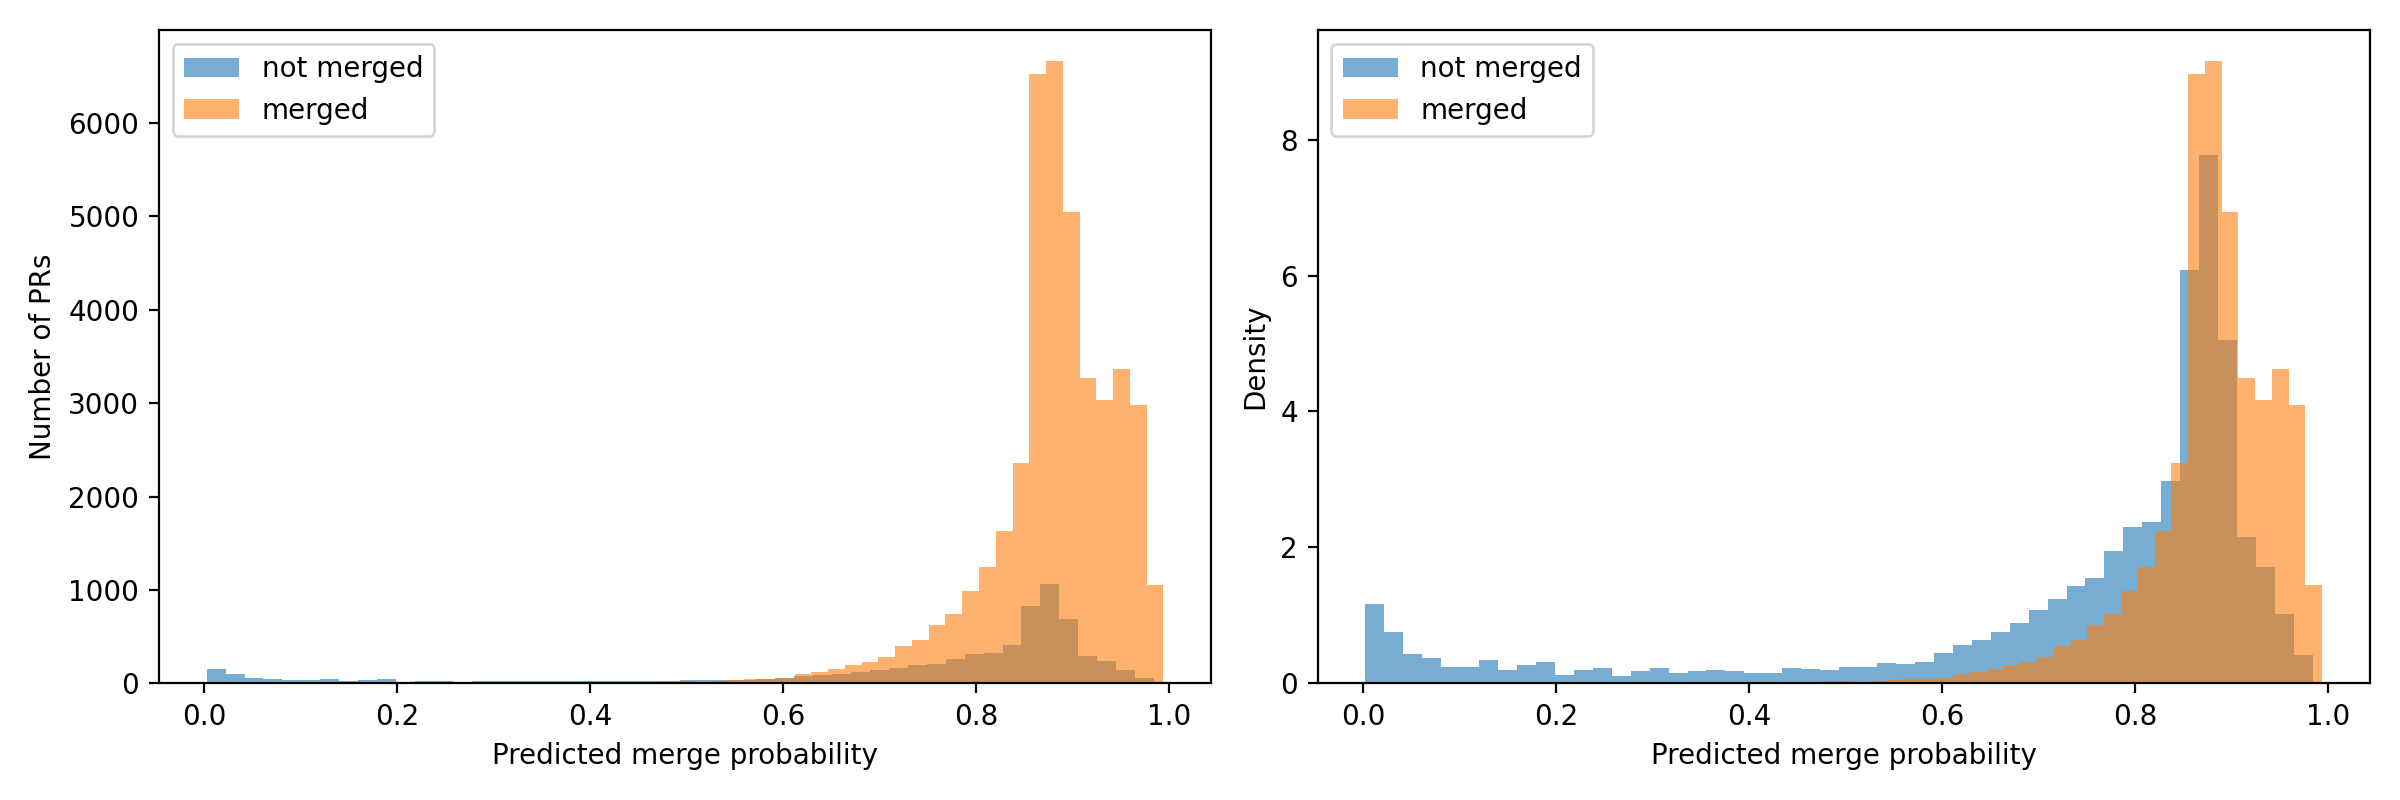
\includegraphics[width=0.95\textwidth]{predicted_probability_distribution.png}
    \caption{Predicted merge probability distribution for merged and non-merged PRs.}
    \label{fig:predicted_probability_distribution}
\end{figure}

Because non-merged PRs are the rarer and more operationally interesting class, additional evaluation was
performed using the risk score

\[
    \text{risk score} = 1 - P(\text{merged}).
\]

Table~\ref{tab:risk_precision} shows that the model is effective at identifying the highest-risk PRs. The
baseline non-merge rate is only 0.1426, but among the top 1\% highest-risk PRs, 0.9939 are actually
non-merged. Even in the top 10\% highest-risk group, the non-merge precision is 0.4581, more than three times
the baseline rate.

\begin{table}[H]
    \centering
    \caption{Risk precision@k for identifying non-merged PRs.}
    \label{tab:risk_precision}
    \begin{tabular}{lrr}
        \toprule
        Risk-ranked subset & Non-merge precision & Baseline non-merge rate \\
        \midrule
        Top 1\% & 0.9939 & 0.1426 \\
        Top 5\% & 0.6257 & 0.1426 \\
        Top 10\% & 0.4581 & 0.1426 \\
        Top 20\% & 0.3325 & 0.1426 \\
        \bottomrule
    \end{tabular}
\end{table}

Threshold analysis further supports this interpretation. Table~\ref{tab:risk_thresholds} shows that
increasing the risk threshold gives higher precision but lower recall. For example, at risk threshold 0.2,
the model flags 15.0\% of PRs, with non-merge precision 0.3827 and recall 0.4028. At threshold 0.5, it flags
2.3\% of PRs, with precision 0.8757 but recall 0.1405.

\begin{table}[H]
    \centering
    \caption{Selected risk-threshold operating points.}
    \label{tab:risk_thresholds}
    \begin{tabular}{rrrrr}
        \toprule
        Risk threshold & Flagged share & Precision & Recall & F1 \\
        \midrule
        0.10 & 0.6659 & 0.1876 & 0.8760 & 0.3091 \\
        0.20 & 0.1501 & 0.3827 & 0.4028 & 0.3925 \\
        0.50 & 0.0229 & 0.8757 & 0.1405 & 0.2421 \\
        0.90 & 0.0083 & 1.0000 & 0.0584 & 0.1104 \\
        \bottomrule
    \end{tabular}
\end{table}

The business interpretation is therefore clear: the model is not a universal automatic decision system, but
it is useful as a prioritization tool. It can surface a small subset of PRs that are unusually likely to
remain unmerged, which could help maintainers inspect blocked, low-fit, or potentially problematic
contributions earlier.

\subsection{Review Process}

The project followed the intended CRISP-DM logic, but the actual work was necessarily data-driven. The main
technical uncertainty was whether GH Archive payloads contained enough information to construct PR lifecycles
and reliable merge labels. Data understanding confirmed that \texttt{PullRequestEvent} contained both opening
and closure actions and that closed PR payloads contained the merge label.

The strongest process decision was to define the analytical grain as one row per pull request. This made the
target, features, and business interpretation consistent. The second important decision was to enforce a
leakage-aware feature policy: all closure-time fields and same-day future events were excluded from the
feature matrix. The third important decision was to evaluate the model as a ranking tool, not only as a hard classifier.

Several limitations remain:

\begin{itemize}
    \item \textbf{Window limitation.} The model uses only PRs opened and closed within the downloaded archive window.
    \item \textbf{Left-censoring.} Repository and actor history are incomplete at the beginning of the sample.
    \item \textbf{Public-data limitation.} Private discussions, CI results, review decisions, and
        maintainers' subjective reasoning are not available.
    \item \textbf{Class imbalance.} Most observed PRs are merged, so default-threshold classification is
        biased toward the positive class.
    \item \textbf{Causal limitation.} The model identifies predictive associations but does not prove why
        maintainers merge or reject PRs.
\end{itemize}

No major omitted step invalidates the current results. The most important limitation is scope: the model
should be presented as a proof-of-concept ranking model for PR outcome risk, not as a production-ready
maintainer decision system.

\subsection{Determine Next Steps}

The current model is approved as an analytical result because it improves over the baseline and provides
strong risk-ranking signal. It should not be deployed as an automated decision-maker.

Possible continuations are:

\begin{enumerate}
    \item \textbf{Use a longer archive window.} This would reduce lifecycle truncation and improve
        repository/actor history quality.
    \item \textbf{Use exact timestamp history.} Instead of previous-day aggregation, features could use
        rolling windows ending exactly at PR opening time.
    \item \textbf{Add early interaction features.} A second scenario could predict after the first 6 or 24
        hours of activity, using comments and reviews after publication but before final closure.
    \item \textbf{Apply time-based validation.} Training on earlier days and testing on later days would
        better approximate deployment.
    \item \textbf{Connect to richer GitHub data.} Review comments, CI statuses, labels, file types, and
        textual PR descriptions could improve explanatory power.
\end{enumerate}

The selected decision is to proceed with the current report as the final course deliverable. The model is
useful for ranking PR merge outcomes under a controlled leakage-aware setup, while the limitations are
explicit enough to avoid overstating the result.

\clearpage
\section{Deployment (CRISP-DM Phase 6)}

The project does not include production deployment. In this course setting, deployment means organizing the analytical result, code, figures, and conclusions in a form that can be reviewed and reused. This is consistent with a report-based deployment scenario: the model is not embedded into a live GitHub workflow, but the result is presented as a reproducible decision-support analysis.

\subsection{Plan Deployment}

The recommended deployment is analytical and report-based rather than automatic operational deployment. The model should be used as a decision-support tool for ranking newly opened pull requests by merge likelihood or non-merge risk. A possible operational scenario is a maintainer dashboard that displays:

\begin{itemize}
    \item a predicted merge probability;
    \item a non-merge risk score;
    \item the most important feature groups, such as repository activity and contributor history;
    \item warnings about data limitations and model scope.
\end{itemize}

The model must not be used to automatically reject, hide, or deprioritize contributors. Its output should support human triage, not replace maintainer judgment. The safest practical use is to surface potentially blocked or low-fit PRs for earlier inspection.

\subsection{Plan Monitoring and Maintenance}

If the approach were used beyond the course setting, monitoring would be required. The following issues should be tracked:

\begin{itemize}
    \item \textbf{Data drift:} GitHub workflows, repository practices, and contributor behavior can change over time.
    \item \textbf{Schema drift:} event payload fields may change or become unavailable.
    \item \textbf{Target drift:} the base merge rate can vary by time period, repository type, and project maturity.
    \item \textbf{Performance drift:} ROC-AUC, PR-AUC, and risk precision@k should be recalculated on newer time windows.
    \item \textbf{Ethical use:} the score should be monitored to ensure that it does not become an automatic gatekeeping mechanism against contributors.
\end{itemize}

A production version should retrain the model on newer and longer archive windows, evaluate with time-based validation, and validate feature extraction after any schema changes. If risk precision drops close to the baseline non-merge rate, the model should be disabled or retrained.

\subsection{Produce Final Report}

The final deliverable of this project is the written CRISP-DM report together with the accompanying code notebooks and generated artifacts. The report summarizes the business objective, data understanding, data preparation pipeline, model comparison, evaluation results, limitations, and recommended next steps.

The final presentation and video are handled separately by the project team. They should present the same central conclusion as the report: public event data available at PR publication time contains useful ranking signal, but the model should be treated as a triage-support tool rather than an automatic decision system.

\subsection{Review Project}

The project successfully produced a leakage-aware PR-level dataset and a ranking model that improves over the majority-class baseline. The main lessons are:

\begin{itemize}
    \item GH Archive is suitable for event-level workflow mining, but the observation window strongly affects lifecycle completeness.
    \item PR merge prediction is heavily imbalanced because most observed PRs are merged.
    \item Default-threshold classification is less informative than ranking-based evaluation for this task.
    \item Repository and contributor history features provide stronger signal than raw PR size alone.
    \item The result is useful for prioritization, but not sufficient for automated maintainer decisions.
\end{itemize}

The main improvement for future versions is to use a longer time range and exact timestamp-based historical windows. This would reduce left-censoring and approximate a real deployment setting more closely.


\end{document}
